% Options for packages loaded elsewhere
\PassOptionsToPackage{unicode}{hyperref}
\PassOptionsToPackage{hyphens}{url}
\PassOptionsToPackage{dvipsnames,svgnames,x11names}{xcolor}
%
\documentclass[
  ignorenonframetext,
]{beamer}
\usepackage{pgfpages}
\setbeamertemplate{caption}[numbered]
\setbeamertemplate{caption label separator}{: }
\setbeamercolor{caption name}{fg=normal text.fg}
\beamertemplatenavigationsymbolsempty
% Prevent slide breaks in the middle of a paragraph
\widowpenalties 1 10000
\raggedbottom
\setbeamertemplate{part page}{
  \centering
  \begin{beamercolorbox}[sep=16pt,center]{part title}
    \usebeamerfont{part title}\insertpart\par
  \end{beamercolorbox}
}
\setbeamertemplate{section page}{
  \centering
  \begin{beamercolorbox}[sep=12pt,center]{part title}
    \usebeamerfont{section title}\insertsection\par
  \end{beamercolorbox}
}
\setbeamertemplate{subsection page}{
  \centering
  \begin{beamercolorbox}[sep=8pt,center]{part title}
    \usebeamerfont{subsection title}\insertsubsection\par
  \end{beamercolorbox}
}
\AtBeginPart{
  \frame{\partpage}
}
\AtBeginSection{
  \ifbibliography
  \else
    \frame{\sectionpage}
  \fi
}
\AtBeginSubsection{
  \frame{\subsectionpage}
}
\usepackage{amsmath,amssymb}
\usepackage{iftex}
\ifPDFTeX
  \usepackage[T1]{fontenc}
  \usepackage[utf8]{inputenc}
  \usepackage{textcomp} % provide euro and other symbols
\else % if luatex or xetex
  \usepackage{unicode-math} % this also loads fontspec
  \defaultfontfeatures{Scale=MatchLowercase}
  \defaultfontfeatures[\rmfamily]{Ligatures=TeX,Scale=1}
\fi
\usepackage{lmodern}
\ifPDFTeX\else
  % xetex/luatex font selection
\fi
% Use upquote if available, for straight quotes in verbatim environments
\IfFileExists{upquote.sty}{\usepackage{upquote}}{}
\IfFileExists{microtype.sty}{% use microtype if available
  \usepackage[]{microtype}
  \UseMicrotypeSet[protrusion]{basicmath} % disable protrusion for tt fonts
}{}
\makeatletter
\@ifundefined{KOMAClassName}{% if non-KOMA class
  \IfFileExists{parskip.sty}{%
    \usepackage{parskip}
  }{% else
    \setlength{\parindent}{0pt}
    \setlength{\parskip}{6pt plus 2pt minus 1pt}}
}{% if KOMA class
  \KOMAoptions{parskip=half}}
\makeatother
\usepackage{xcolor}
\newif\ifbibliography
\usepackage{graphicx}
\makeatletter
\def\maxwidth{\ifdim\Gin@nat@width>\linewidth\linewidth\else\Gin@nat@width\fi}
\def\maxheight{\ifdim\Gin@nat@height>\textheight\textheight\else\Gin@nat@height\fi}
\makeatother
% Scale images if necessary, so that they will not overflow the page
% margins by default, and it is still possible to overwrite the defaults
% using explicit options in \includegraphics[width, height, ...]{}
\setkeys{Gin}{width=\maxwidth,height=\maxheight,keepaspectratio}
% Set default figure placement to htbp
\makeatletter
\def\fps@figure{htbp}
\makeatother
\setlength{\emergencystretch}{3em} % prevent overfull lines
\providecommand{\tightlist}{%
  \setlength{\itemsep}{0pt}\setlength{\parskip}{0pt}}
\setcounter{secnumdepth}{-\maxdimen} % remove section numbering
\newcommand{\columnsbegin}{\begin{columns}}
\newcommand{\columnsend}{\end{columns}}
\makeatletter
\def\insertnavigation#1{%
  \vbox{{%
    \usebeamerfont{section in head/foot}\usebeamercolor[fg]{section in head/foot}%
    \beamer@xpos=0\relax%
    \beamer@ypos=1\relax%
    \beamer@ypos@offset=0\relax%
    \hbox to #1{\hskip.3cm\setbox\beamer@sectionbox=\hbox{\kern1sp}%
      \ht\beamer@sectionbox=1.875ex%
      \dp\beamer@sectionbox=0.75ex%
        \hskip-1.875ex plus-1fill%
        \global\beamer@section@min@dim\z@
        \dohead%
        \beamer@section@set@min@width
      \box\beamer@sectionbox\hfil\hskip.3cm\hskip0pt plus1filll}%
  }}} 
\makeatother
\DeclareMathAlphabet{\mathams}{U}{msb}{m}{n}
\newcommand{\ex}{\mathams{E}}
\usepackage{tcolorbox}
\newtcolorbox{codebox}{enhanced,colback=shadecolor,colframe=orange,boxrule=.2pt, arc=0pt, width=\paperwidth, enlarge left by=-10mm}
\AtBeginSection{}
\useoutertheme{miniframes}
\setbeamertemplate{frametitle}{\vskip0.3cm\usebeamerfont*{frametitle}\insertframetitle\vskip-1.5ex\begin{beamercolorbox}[colsep=0.2pt, wd=\textwidth]{lower separation line head}\end{beamercolorbox}}
\setbeamercolor{lower separation line head}{bg=orange}
\definecolor{shadecolor}{RGB}{200, 200, 200}
\hypersetup{colorlinks,citecolor=orange,filecolor=red,linkcolor=brown,urlcolor=blue}
\definecolor{green}{RGB}{48, 69, 41}
\definecolor{darkorange}{RGB}{255, 150, 0}
\definecolor{gray}{RGB}{100, 100, 100}
\setbeamercolor{itemize item}{fg=orange}
\setbeamercolor{itemize subitem}{fg=orange}
\setbeamercolor{enumerate item}{fg=orange}
\setbeamercolor{enumerate subitem}{fg=orange}
\tcbuselibrary{skins}
\usepackage{emoji}
\ifLuaTeX
  \usepackage{selnolig}  % disable illegal ligatures
\fi
\IfFileExists{bookmark.sty}{\usepackage{bookmark}}{\usepackage{hyperref}}
\IfFileExists{xurl.sty}{\usepackage{xurl}}{} % add URL line breaks if available
\urlstyle{same}
\hypersetup{
  pdftitle={Introduction},
  pdfauthor={Bert van der Veen},
  colorlinks=true,
  linkcolor={Maroon},
  filecolor={Maroon},
  citecolor={Blue},
  urlcolor={orange},
  pdfcreator={LaTeX via pandoc}}

\title{Introduction}
\author{Bert van der Veen}
\date{}
\institute{Department of Mathematical Sciences, NTNU}

\begin{document}
\frame{\titlepage}

\hypertarget{welcome}{%
\section{\texorpdfstring{Welcome!
\emoji{smile}}{Welcome! }}\label{welcome}}

\begin{frame}{Welcome! \emoji{smile}}
\center


\includegraphics[width=0.6\textwidth,height=\textheight]{audience.png}
\end{frame}

\hypertarget{outline}{%
\section{Outline}\label{outline}}

\begin{frame}{Outline}
\href{https://github.com/BertvanderVeen/GLM-workshop}{See github for all
material}

Sessions from 14:00 to 20:00 (Monday to Thursday), 14:00 to 18:00 on
Friday (Berlin time). Sessions will consist of a mix of lectures,
in-class discussion, and practical exercises / case studies over Slack
and Zoom.

\begin{itemize}
\tightlist
\item
  Monday: Introduction and Basics, do a taskcard in introduction?
\item
  Tuesday: Multiple linear regression (ANOVA, ANCOVA) + GLM introduction
\item
  Wednesday: Binomial regression, model comparison
\item
  Thursday: Discrete responses (Poisson, NB) and other useful models
  (e.g., beta)
\item
  Friday: Bring your own data, looking beyond (GLMMs, GAMs, Bayesian
  statistics, and such)
\end{itemize}
\end{frame}

\begin{frame}{How we will do it}
\protect\hypertarget{how-we-will-do-it}{}
Lectures of about 45 minutes \newline Practicals of about 45 minutes:
datasets and R

\begin{itemize}
\tightlist
\item
  Practical ``tasks'' serve as guideline, not as exhaustive exercise
\item
  I do not provide a lot of \texttt{R} code. We will figure that out
  together!
\end{itemize}
\end{frame}

\begin{frame}{Disclaimer}
\protect\hypertarget{disclaimer}{}
A \tiny small \normalsize amount of \tiny \color{red}{maths}


\includegraphics[width=0.5\textwidth,height=\textheight]{stats.jpeg}

\vfill

\hfill  This is a statistics workshop after all \normalsize
\end{frame}

\begin{frame}{What I hope you take away}
\protect\hypertarget{what-i-hope-you-take-away}{}
\begin{enumerate}
\tightlist
\item
  There are many details you will forget, that is fine (you might recall
  them later)
\item
  Generalised Linear Models are very useful, and easy to use
\item
  Maths can be useful/stats can be useful
\item
  You pick the tools you want to work with
\end{enumerate}

\center


\includegraphics[width=0.4\textwidth,height=\textheight]{model.png}
\end{frame}

\begin{frame}{Detailed outline today}
\protect\hypertarget{detailed-outline-today}{}
\begin{itemize}
\item
  Who am I, who are you
\item
  Brief reminder of R programming
\item
  Reminder of foundational statistical concepts (sampling theory)
\item
  Introduction to linear models
\item
  15 minute break 15:45-16:00
\item
  45 minute break 17:45-18:30
\item
  2 Lectures/presentations
\item
  2 Practicals based on simulated data

  \begin{itemize}
  \tightlist
  \item
    Tomorrow we start with real data
  \end{itemize}
\end{itemize}
\end{frame}

\hypertarget{logistics}{%
\section{Logistics}\label{logistics}}

\begin{frame}{Logistics}
\href{https://github.com/BertvanderVeen/GLM-workshop}{All material on
github}

Please make sure you've downloaded data and updated R/packages
\end{frame}

\begin{frame}{\texttt{R}-packages}
\protect\hypertarget{packages}{}
\columnsbegin
\column{0.5\textwidth}

\begin{itemize}
\tightlist
\item
  car
\item
  visreg
\item
  effects
\item
  emmeans
\item
  DHARMa
\item
  MuMIn
\item
  performance
\item
  stargazer
\item
  apaTables
\item
  ggplot2
\item
  AICcmodavg
\end{itemize}

\column{0.5\textwidth}

\textcolor{red}{New}

\begin{itemize}
\tightlist
\item
  glmtoolbox
\item
  patchwork
\item
  DescTools
\item
  VGAM/glmmTMB
\item
  tweedie
\item
  statmod
\item
  arm
\end{itemize}

\columnsend
\end{frame}

\begin{frame}{Resources}
\protect\hypertarget{resources}{}
\begin{itemize}
\item
  \href{https://wiki.math.ntnu.no/st2304/2024v/start}{ST2304} by Bob
  O'Hara and Emily Simmonds
\item
  \href{https://theoreticalecology.github.io/AdvancedRegressionModels}{Florian
  Hartig's online book}
\item
  \href{https://statistics4ecologists-v2.netlify.app/}{John Fieberg's
  online book}
\item
  \href{https://www.highstat.com/index.php/our-books?view=article\&id=21\&catid=18}{Zuur
  et al.~2013} or
  \href{https://www.highstat.com/index.php/our-books?view=article\&id=17\&catid=18}{Zuur
  et al.~2009}
\item
  \href{https://www.taylorfrancis.com/books/mono/10.1201/9780203753736/generalized-linear-models-mccullagh}{McCullagh
  and Nelder 1989}
\item
  \href{https://www.taylorfrancis.com/books/mono/10.1201/9781315370279/generalized-additive-models-simon-wood}{Wood
  2017}
\item
  \href{https://link.springer.com/book/10.1007/978-1-4419-0118-7}{Dunn
  and Smyth 2021}
\item
  \href{https://onlinelibrary.wiley.com/doi/book/10.1002/0471249688}{Agresti
  1990}
\end{itemize}
\end{frame}

\hypertarget{introducions}{%
\section{IntroducionS}\label{introducions}}

\begin{frame}{Who am I, and what do I do?}
\protect\hypertarget{who-am-i-and-what-do-i-do}{}
\columnsbegin
\column{0.5\textwidth}


\includegraphics{statistician.jpg}

\column{0.5\textwidth}

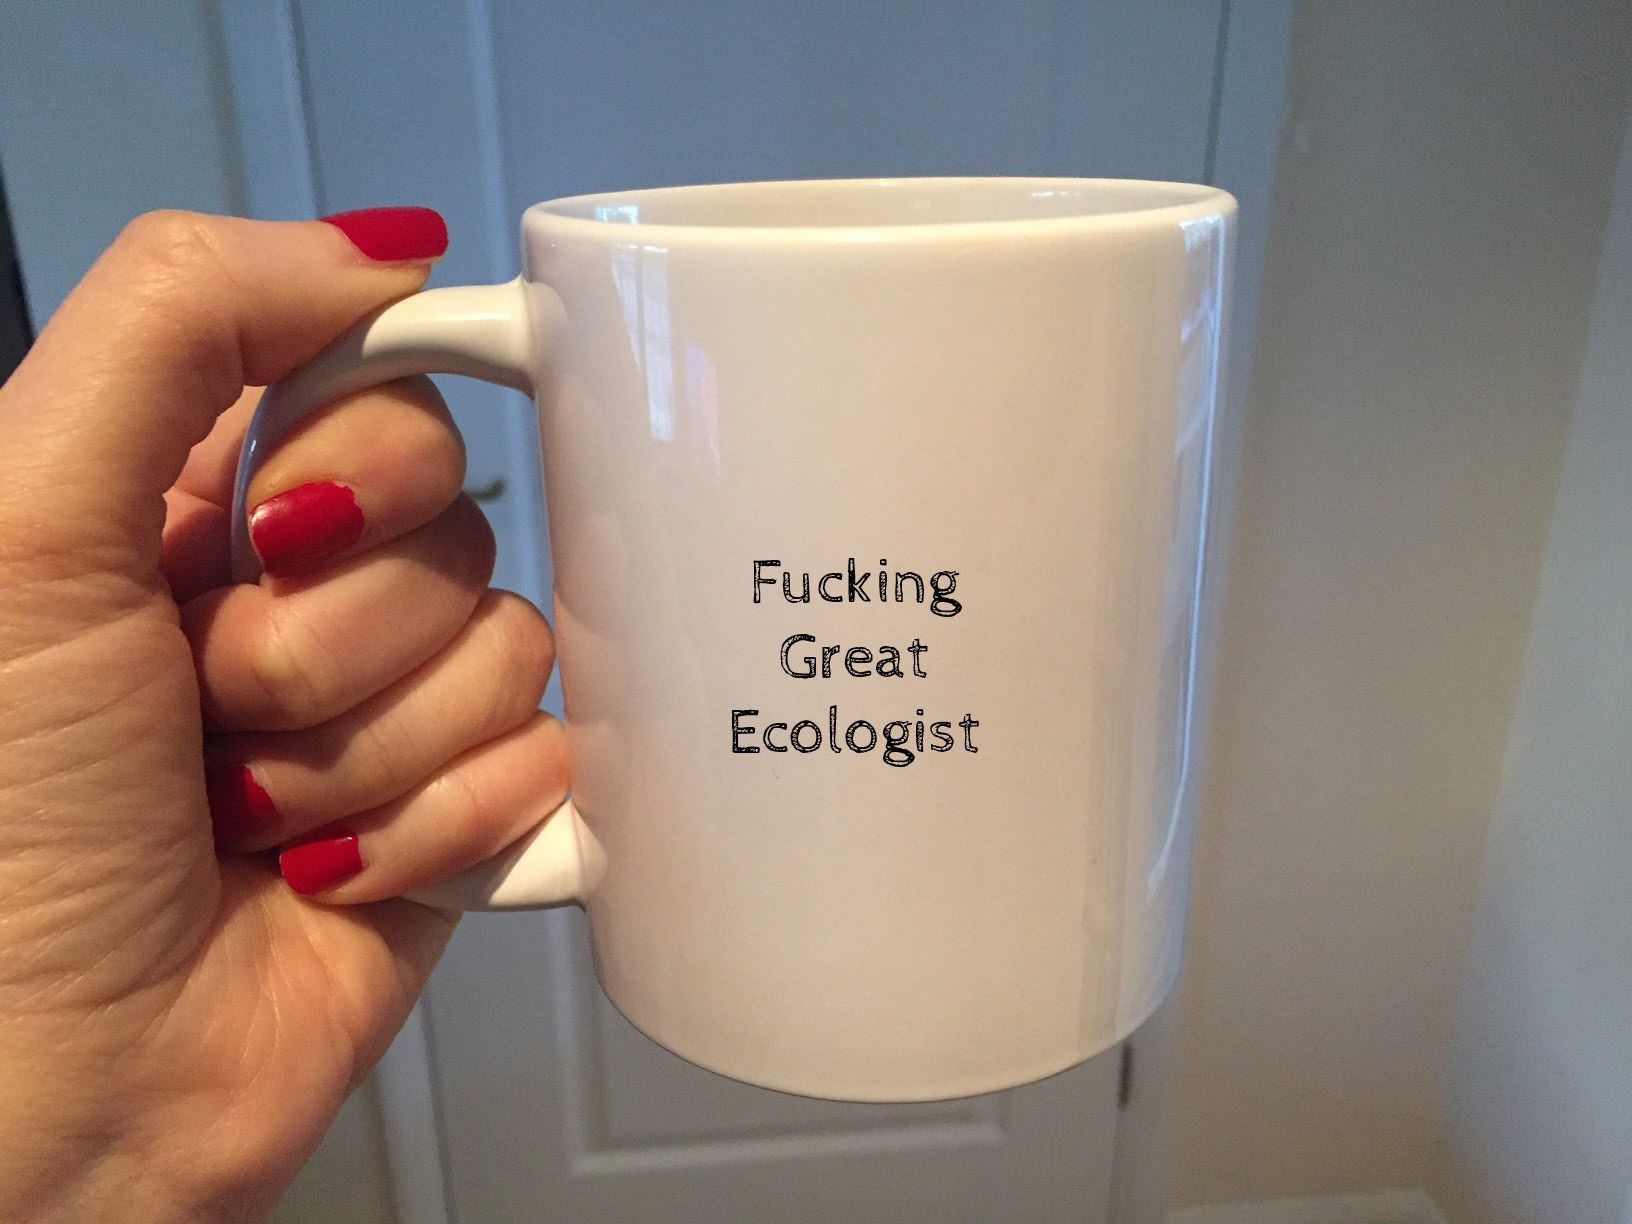
\includegraphics{ecologist2.jpg}

\columnsend
\end{frame}

\begin{frame}{Who are you, and what do you do?}
\protect\hypertarget{who-are-you-and-what-do-you-do}{}
\center


\includegraphics[width=0.5\textwidth,height=\textheight]{introductions.jpg}
\end{frame}

\end{document}
